
\section{Висновок}
\setlength{\parindent}{4em}
\qquad У даній роботі ми провели дослідження дифракційної гратки і використали отримане значення для визначення довжини хвилі спектру ртуті. Отримані значення досить близькі до реальних, що може свідчити про правильність експерименту і правильність розрахунків. Отримані результати:
\begin{figure}[ht]

\centering

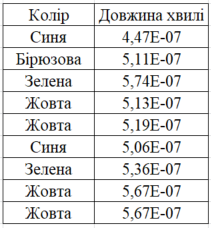
\includegraphics[width=0.6\linewidth]{Pics/tabl5.png}

\label{table1}

\end{figure}
